\documentclass{article}

%-------------------------%
% PREAMBUŁA --------------%
%-------------------------%
\usepackage[utf8]{inputenc}
\usepackage[OT4]{polski}
\usepackage{caption}
\usepackage{amsmath}
\usepackage{tikz}
\usepackage{subcaption}
\usepackage{tabularx}
\usepackage{caption}
\usepackage{array}
\usepackage{hyperref}
\usepackage{graphicx}
\usepackage{fancyhdr}
\usepackage[justification=centering]{caption}
\usepackage[margin=60pt]{geometry}
\usepackage{longtable}



%\usepackage[T1]{fontenc}
%\usepackage{amsthm}
%\theoremstyle{plain}
%\usepackage{enumitem}
%\captionsetup[table]{skip=-4pt}
%\usepackage{tabulary}
%\usepackage{sidecap}
%\usepackage{gensymb}
%\usepackage{wrapfig}
%\usepackage{lastpage}
%\usepackage{gensymb}
%\usepackage{lipsum}
%\pagestyle{fancy}


\newlength{\RoundedBoxWidth}
\newsavebox{\GrayRoundedBox}
\newenvironment{GrayBox}[1][\dimexpr\textwidth-4.5ex]%
   {\setlength{\RoundedBoxWidth}{\dimexpr#1}
    \begin{lrbox}{\GrayRoundedBox}
       \begin{minipage}{\RoundedBoxWidth}}%
   {   \end{minipage}
    \end{lrbox}
    \begin{center}
    
\begin{tikzpicture}%
       \draw node[draw=black,fill=black!1,rounded corners,%
             inner sep=2ex,text width=\RoundedBoxWidth]%
             {\usebox{\GrayRoundedBox}};
    \end{tikzpicture}
    \end{center}}

%------- Typy kolumn do ustawiania szerokości ------- %
\newcolumntype{L}[1]{>{\raggedright\let\newline\\\arraybackslash\hspace{0pt}}m{#1}}
\newcolumntype{C}[1]{>{\centering\let\newline\\\arraybackslash\hspace{0pt}}m{#1}}
\newcolumntype{R}[1]{>{\raggedleft\let\newline\\\arraybackslash\hspace{0pt}}m{#1}}








\begin{document}

%-------------------------%
%Tabela nagłówkowa -------%
%-------------------------%

\begin{table}[h]
\begin{tabular}{|l|l|l|l|l|l|}
\hline
\begin{tabular}[c]{@{}l@{}}
Wydział:\\ WFiIS\end{tabular} &
\multicolumn{2}{l|}{\begin{tabular}[c]{@{}l@{}}
Imię i nazwisko:\\ 1. Axel Zuziak\\ 2. Marcin Węglarz \end{tabular}} 
& Rok \textbf{II}         
& Grupa \textbf{B}          
& Zespół \textbf{03}      \\ \hline
\textbf{\begin{tabular}[c]{@{}l@{}}
LABOLATORIUM\\ TECHNIK \\ JĄDROWYCH\end{tabular}} &
\multicolumn{4}{l|}{ Temat:\textbf{ Wyznaczanie czasu połowicznego rozpadu
		izotopów krótkotrwałych.} }                                                                                                                       & \multicolumn{1}{c|}{\begin{tabular}[c]{@{}c@{}}
Nr ćwiczenia\\ \textbf{06}
\end{tabular}} \\ \hline
\begin{tabular}[c]{@{}c@{}}
Data wykonania:\\ 04.03.2015
\end{tabular} &
\begin{tabular}[c]{@{}c@{}}
 Data oddania:\\ 18.03.2015
\end{tabular} &
\begin{tabular}[c]{@{}c@{}}
Zwrot do poprawy: \\ 
\end{tabular}                                 
& 
\begin{tabular}[c]{@{}c@{}}
Data oddania: \\ 
\end{tabular}&
\begin{tabular}[c]{@{}c@{}}
Data zaliczenia:\\
\end{tabular}& 
\begin{tabular}[c]{@{}c@{}}
OCENA:\\
\end{tabular}       
\\ & & & & & \\ \hline
\end{tabular}
\end{table}
%-----Koniec tabeli------

%WSTĘP++++++++++++++++++++++++++++++++++++++++++++++++++++

\section{Czas połowicznego rozpadu srebra.}
\subsection{Cel ćwiczenia.}
   Celem ćwiczenia jest doświadczalne wyznaczenie czasu połowicznego rozpadu płytki srebra zaaktywowanej wcześniej przy pomocy neutronów.

\subsection{Wstęp.}
Doświadczalne wyznaczenie czasu połowicznego rozpadu poprzez narysowanie krzywej rozpadu jest możliwe dla izotopów o krótkim czasie życia (czas połowicznego rozpadu rzędu kilkudziesięciu sekund lub kilku minut).
Przykładami takich izotopów mogą być aktywowane izotopy srebra.

W przyrodzie srebro występuje w postaci dwóch stabilnych izotopów: $^{107}$Ag (51.35\%) oraz $^{109}$Ag (48.65\%). Pod wpływem bombardowania neutronami (termicznymi lub szybkimi) srebro ulega aktywacji poprzez pochłonięcie neutronu:\\
\[^{107}\text{Ag} + \text{n} \to ^{108}\text{Ag} + \gamma
\]
\[^{109}\text{Ag} + \text{n} \to ^{110}\text{Ag} + \gamma
\]\\\\
Oprócz powyższych izotopów powstają jeszcze $^{108m}$Ag oraz $^{110m}$Ag jednak ich czasy połowicznego rozpadu to odpowiednio 418 lat oraz 250 dni, więc nie wpływają one na wyniki naszego doświadczenia.\\
Powstałe w wyniku aktywacji izotopy mają czas połowicznego rozpadu (tablicowy \cite{1}) równy 2.37 min dla $^{108}$Ag oraz 24.6 s dla $^{110}$Ag, co w dalszej części doświadczenia wyznaczano. Oba izotopy ulegają rozpadowi $\beta ^-$. \\\\
Powyższe rozpady opisuje prawo rozpadu promioniotwórczego:
\begin{equation}
N(t) = N_0 \exp^{-\lambda t}
\end{equation}
Po przekształceniu możemy je zapisać w postaci:
\begin{equation}
\ln N = -\lambda t + \ln N_0
\label{wz_rozpad_log}
\end{equation}
Z powyższego równania wynika, że dla rozpadu pojedynczego izotopu narysowany w skali półlogarytmicznej wykres liczby rozpadów od czasu powinien być linią prostą. Wyznaczając współczynnik kierunkowy tej prostej oraz korzystając z definicji czasu połowicznego rozpadu możemy go wyznaczyć jako:
\begin{equation}
\tau = \frac{\ln 2}{\lambda}
\label{wz_tau}
\end{equation}
Gdzie:\\
$\tau$ - czas połowicznego rozpadu\\
$\lambda $ - stała rozpadu wyznaczona jako współczynnik nachylenia prostej\\

W przypadku, gdy w badanej próbce znajduję się kilka izotopów wykorzystujemy różnicę w czasach połowicznego rozpadu ( po czasie około 3.5$\tau _1$ pierwszy z izotopów całkowicie się rozpadnie przy czym ciągle będziemy rejestrować rozpady drugiego izotopu). Narysowany w skali półlogarytmicznej wykres powinien wyglądać mniej więcej tak jak ten na Rysunku \ref{schemat}. \\
Krzywa 1 na rysunku reprezentuję wyznaczoną krzywą, celem znalezienia prostej $2$ należy wyznaczyć (np. metodą najmniejszych kwadratów) równanie prostej $1'$, a następnie ekstrapolować ją punktu $t=0$. Jeżeli przez $t_1$ oznaczymy czas, w którym izotop o krótszym czasie życia uległ całkowitemu rozpadowi, to prostą $1'$ będziemy dopasowywać do punktów zaczynających się od tego właśnie punktu. Kolejnym krokiem jest odjęcie prostej $1'$ od danych pomiarowych i do otrzymanych punktów z przedziału od $t=0$ do $t_1$ ponownie dopasowujemy prostą.\\
Otrzymane proste to proste rozpadu poszczególnych izotopów w skali półlogarytmicznej, czasy ich połowicznego rozpadu wyznaczamy ze wzoru (\ref{wz_tau})

\begin{figure}[h]
	\centering
	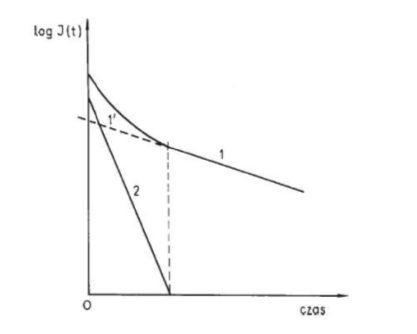
\includegraphics[width=0.7\textwidth]{images/schemat.png}
	\caption{Schemat wykresu półlogarytmicznego dla rozpadu dwóch izotopów różniących się czasami połowicznego rozpadu.}
	\label{schemat}
\end{figure}



\subsection{Wykonanie ćwiczenia.}
Doświadczenie rozpoczęto od włożenia srebrnej płytki do źródła neutronów na czas 10 minut.\\
Następnie po upływie tego czasu bardzo szybko (około 20s upłynęło od wyjęcia płytki do rozpoczęcia pomiarów) wyjęto płytkę i umieszczono w detektorze  rozpoczynając pomiary. Liczbę zliczeń notowano w odstępie 6 sekund, wyniki przedstawia tabela \ref{wyniki_dat} oraz wykres przedstawiony na Rysunku \ref{wykres_zliczenia_czas}. Czas $t_1$ całkowitego rozpadu srebra $^{110}$Ag oszacowano na 150s.\\
Do dalszych obliczeń przyjęto, że wielkości związane z $^{108}$Ag będą miały indeks 1 natomiast związane z $^{110}$Ag indeks 2.\\

\begin{figure}[h!]
	\fontsize{6}{8}\selectfont % zmniejszam czcionke
	\centering
	\resizebox{1.0\textwidth}{!}{% GNUPLOT: LaTeX picture with Postscript
\begingroup
  \makeatletter
  \providecommand\color[2][]{%
    \GenericError{(gnuplot) \space\space\space\@spaces}{%
      Package color not loaded in conjunction with
      terminal option `colourtext'%
    }{See the gnuplot documentation for explanation.%
    }{Either use 'blacktext' in gnuplot or load the package
      color.sty in LaTeX.}%
    \renewcommand\color[2][]{}%
  }%
  \providecommand\includegraphics[2][]{%
    \GenericError{(gnuplot) \space\space\space\@spaces}{%
      Package graphicx or graphics not loaded%
    }{See the gnuplot documentation for explanation.%
    }{The gnuplot epslatex terminal needs graphicx.sty or graphics.sty.}%
    \renewcommand\includegraphics[2][]{}%
  }%
  \providecommand\rotatebox[2]{#2}%
  \@ifundefined{ifGPcolor}{%
    \newif\ifGPcolor
    \GPcolortrue
  }{}%
  \@ifundefined{ifGPblacktext}{%
    \newif\ifGPblacktext
    \GPblacktextfalse
  }{}%
  % define a \g@addto@macro without @ in the name:
  \let\gplgaddtomacro\g@addto@macro
  % define empty templates for all commands taking text:
  \gdef\gplbacktext{}%
  \gdef\gplfronttext{}%
  \makeatother
  \ifGPblacktext
    % no textcolor at all
    \def\colorrgb#1{}%
    \def\colorgray#1{}%
  \else
    % gray or color?
    \ifGPcolor
      \def\colorrgb#1{\color[rgb]{#1}}%
      \def\colorgray#1{\color[gray]{#1}}%
      \expandafter\def\csname LTw\endcsname{\color{white}}%
      \expandafter\def\csname LTb\endcsname{\color{black}}%
      \expandafter\def\csname LTa\endcsname{\color{black}}%
      \expandafter\def\csname LT0\endcsname{\color[rgb]{1,0,0}}%
      \expandafter\def\csname LT1\endcsname{\color[rgb]{0,1,0}}%
      \expandafter\def\csname LT2\endcsname{\color[rgb]{0,0,1}}%
      \expandafter\def\csname LT3\endcsname{\color[rgb]{1,0,1}}%
      \expandafter\def\csname LT4\endcsname{\color[rgb]{0,1,1}}%
      \expandafter\def\csname LT5\endcsname{\color[rgb]{1,1,0}}%
      \expandafter\def\csname LT6\endcsname{\color[rgb]{0,0,0}}%
      \expandafter\def\csname LT7\endcsname{\color[rgb]{1,0.3,0}}%
      \expandafter\def\csname LT8\endcsname{\color[rgb]{0.5,0.5,0.5}}%
    \else
      % gray
      \def\colorrgb#1{\color{black}}%
      \def\colorgray#1{\color[gray]{#1}}%
      \expandafter\def\csname LTw\endcsname{\color{white}}%
      \expandafter\def\csname LTb\endcsname{\color{black}}%
      \expandafter\def\csname LTa\endcsname{\color{black}}%
      \expandafter\def\csname LT0\endcsname{\color{black}}%
      \expandafter\def\csname LT1\endcsname{\color{black}}%
      \expandafter\def\csname LT2\endcsname{\color{black}}%
      \expandafter\def\csname LT3\endcsname{\color{black}}%
      \expandafter\def\csname LT4\endcsname{\color{black}}%
      \expandafter\def\csname LT5\endcsname{\color{black}}%
      \expandafter\def\csname LT6\endcsname{\color{black}}%
      \expandafter\def\csname LT7\endcsname{\color{black}}%
      \expandafter\def\csname LT8\endcsname{\color{black}}%
    \fi
  \fi
  \setlength{\unitlength}{0.0500bp}%
  \begin{picture}(7370.00,5102.00)%
    \gplgaddtomacro\gplbacktext{%
      \csname LTb\endcsname%
      \put(550,704){\makebox(0,0)[r]{\strut{}$1$}}%
      \csname LTb\endcsname%
      \put(550,1294){\makebox(0,0)[r]{\strut{}$2$}}%
      \csname LTb\endcsname%
      \put(550,1885){\makebox(0,0)[r]{\strut{}$3$}}%
      \csname LTb\endcsname%
      \put(550,2475){\makebox(0,0)[r]{\strut{}$4$}}%
      \csname LTb\endcsname%
      \put(550,3066){\makebox(0,0)[r]{\strut{}$5$}}%
      \csname LTb\endcsname%
      \put(550,3656){\makebox(0,0)[r]{\strut{}$6$}}%
      \csname LTb\endcsname%
      \put(550,4247){\makebox(0,0)[r]{\strut{}$7$}}%
      \csname LTb\endcsname%
      \put(550,4837){\makebox(0,0)[r]{\strut{}$8$}}%
      \csname LTb\endcsname%
      \put(682,484){\makebox(0,0){\strut{}$0$}}%
      \csname LTb\endcsname%
      \put(1468,484){\makebox(0,0){\strut{}$100$}}%
      \csname LTb\endcsname%
      \put(2255,484){\makebox(0,0){\strut{}$200$}}%
      \csname LTb\endcsname%
      \put(3041,484){\makebox(0,0){\strut{}$300$}}%
      \csname LTb\endcsname%
      \put(3828,484){\makebox(0,0){\strut{}$400$}}%
      \csname LTb\endcsname%
      \put(4614,484){\makebox(0,0){\strut{}$500$}}%
      \csname LTb\endcsname%
      \put(5400,484){\makebox(0,0){\strut{}$600$}}%
      \csname LTb\endcsname%
      \put(6187,484){\makebox(0,0){\strut{}$700$}}%
      \csname LTb\endcsname%
      \put(6973,484){\makebox(0,0){\strut{}$800$}}%
      \put(176,2770){\rotatebox{-270}{\makebox(0,0){\strut{}log(N)}}}%
      \put(3827,154){\makebox(0,0){\strut{}Czas [s]}}%
    }%
    \gplgaddtomacro\gplfronttext{%
      \csname LTb\endcsname%
      \put(5986,4664){\makebox(0,0)[r]{\strut{}$^{108}$Ag}}%
      \csname LTb\endcsname%
      \put(5986,4444){\makebox(0,0)[r]{\strut{}$^{110}$Ag}}%
    }%
    \gplbacktext
    \put(0,0){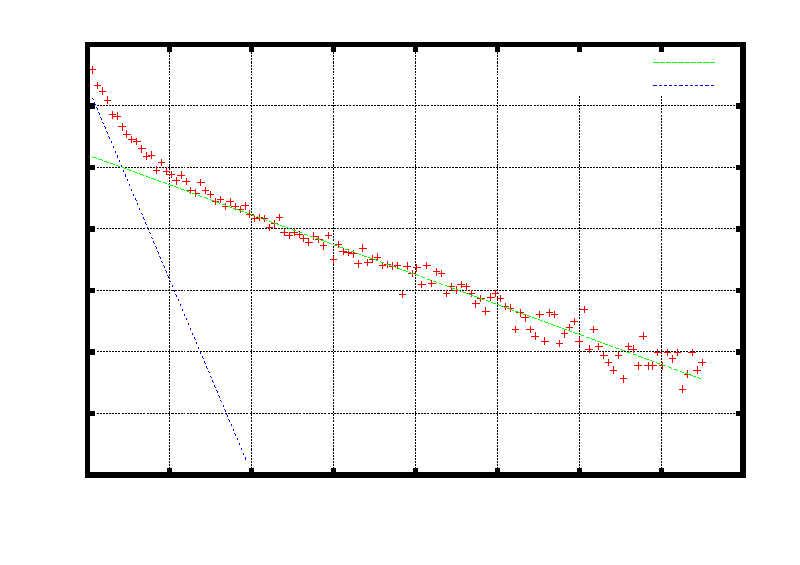
\includegraphics{srebro}}%
    \gplfronttext
  \end{picture}%
\endgroup
}	
	
	\caption{Częstość zliczeń w skali logarytmicznej z naniesionymi prostymi odpowiadającymi rozpadom poszczególnych izotopów srebra.}
	\label{wykres_zliczenia_czas}
\end{figure}

Do danych pomiarowych dla czasu $t$ większego od 150 sekund dopasowano prostą odpowiadającą rozpadowi $^{108}$Ag : \\
\[a_1 = -4.864 \pm 0.085 \cdot 10^{-3}
\]
\[	b_1 = 6.205 \pm 0.041
\]
Porównując współczynnik $a_1$ ze wzorem (\ref{wz_rozpad_log}) otrzymujemy:\\
$\lambda _1 =  4.864 \pm 0.085 \cdot 10^{-3}$\\\\

W kolejnym kroku odjęto od danych pomiarowych wartości funkcji $a_1 x + b_1$ i do otrzymanych punktów w zakresie [0:150] sekund dopasowano prostą odpowiadającą rozpadowi $^{110}$Ag :
\[a_2 = -0.0314 \pm 0.0017
\]
\[b_2 = 7.32 \pm 0.13
\]
Ponownie porównując prostą ze wzorem (\ref{wz_rozpad_log}) otrzymujemy:\\
$\lambda _2 = 0.0314 \pm 0.0017$

W ostatnim kroku korzystając ze wzoru (\ref{wz_tau}) oraz z prawa przenoszenia niepewności pomiarowej wyznaczono czasy połowicznego rozpadu.
\begin{equation}
u(\tau) = \sqrt{ \Big[ \frac{-\ln 2}{\lambda ^2}u(\lambda) \Big]^2 }
\label{wz_niepewnosc}
\end{equation}

\noindent
Wyliczone wartości dla $^{108}$Ag:\\
\[\tau _1 = 142.5 \pm 2.5\text{ s}
\]
\[\tau _{1tab} = 142.2 \text{s}
\]
\\\\
oraz dla $^{110}$Ag:\\
\[\tau _2 = 22.1 \pm 1.2 \text{s}
\]
\[\tau _{2tab} = 24.6 \text{s}
\]


\subsection{Wnioski.}
Wartości możemy uznać za równe jeżeli moduł z różnicy tych wartości jest mniejszy od niepewności wyznaczenia wartości pomnożonej przez stałą $k$ (przyjmujemy $k$=2). \\
$|\tau _1 -\tau _{1tab}| = 0.3$  $k\cdot u(\tau _1)=  5$ \\
$0.3 < 5$\\\\
Tak więc dla $^{108}$Ag wyniki uzyskane doświadczalnie są zgodne z wartościami tablicowymi.\\\\

\noindent
$|\tau _2 -\tau _{2tab}| = 2.5$  $k\cdot u(\tau _2)=  2.4$ \\
$2.5 \not< 2.4$\\\\
Wartości wyznaczone dla $^{110}$Ag nie są zgodne z wartościami tablicowymi dla $k$=2, jednak jak widać różnica jest niewielka. Wpływ na wynik ma również bardzo krótki czas życia $^{110}$Ag, być może gdyby szybciej umieszczono próbkę w detektorze udało by się dokładniej wyznaczyć czas połowicznego rozpadu i z większą dokładnością.  \\
Przedstawiona powyżej metoda jest dobrym sposobem na wyznaczenie czasu połowicznego rozpadu izotopów których czas życia jest niewielki. Szczególnie dokładny wynik otrzymaliśmy dla izotopu $^{108}$Ag.
















\end{document}





%http://nucleardata.nuclear.lu.se/toi/
%do bibliografii






